\documentclass{article}
\usepackage[margin=0.73in]{geometry}
\usepackage{amsmath}
\usepackage{amssymb}
\usepackage{graphicx}
\usepackage{float}
\usepackage{hyperref}

\title{Report for Programming Assignment 1}
\author{Vishwak Srinivasan\\
\texttt{CS15BTECH11043}}
\date{}

\begin{document}
\maketitle

\section*{Instructions for examining the programs}
\begin{itemize}
\item There are three important programs: \texttt{fixed\_step\_size.py} for fixed step size (Question 2), \texttt{backtracking\_ls.py} for backtracing line search (Question 3) and \texttt{inv\_step\_size.py} for learning rate = \(\frac{1}{k}\) (Question 4).
\item All of the above mentioned files depend on \texttt{NumPy} and a module \texttt{functions.py}, included with these programs.
\item To test a program, run \texttt{python3 <name\_of\_the\_program> -h}. The options are there for your convenience.
\item Since analytically arriving at a solution for \(f_{LL}\) was not possible, I wrote a smaller program to find the roots of partial derivatives using the Newton-Raphson Method \texttt{newton\_raphson.py}. 
\item The plots were generated using \texttt{GNUplot}. The plots can be obtained by running \texttt{gnuplot plotter.gnuplot}.
\end{itemize}

\section*{Main Report}
\begin{flushleft}
The ``special" functions in consideration for this assignment were:
\begin{gather*}
f_{Q}(x, y) = 1.125x^2 + 0.5xy + 0.75y^2 + 2x + 2y \\
f_{LL}(x, y) = 0.5(x^2 + y^2) + 50\log\left(1 + e^{-0.5y}\right) + 50\log\left(1 + e^{0.2x}\right) \\
f_{H}(x, y) = 0.1(x^2 + y - 11)^2 + 0.1(x + y^2 - 7)^2 \\
f_{R}(x, y) = 0.002(1 - x)^2 + 0.2(y - x^2)^2
\end{gather*}

\begin{itemize}
\item In the domain of consideration i.e., \([-6, 6]\times[-6, 6]\) for \(f_{Q}, f_{LL} \text{ \& } f_{H}\) and \([-3, 3] \times [-6, 6]\) for \(f_{R}\) --- \(f_{Q}\) and \(f_{LL}\) were found to convex, and \(f_{H}\) and \(f_{R}\) were found to be non-convex. All these inferences were based of the surfaces plotted.
\item \(f_{Q}\) and \(f_{LL}\) have 1 minimum each, whereas \(f_{H}\) has 4 local minima and 1 local maximum. The problem with \(f_{R}\) is the existence of a valley like structure.
\end{itemize}

\begin{figure}[H]
\begin{minipage}{0.45\linewidth}
\centering
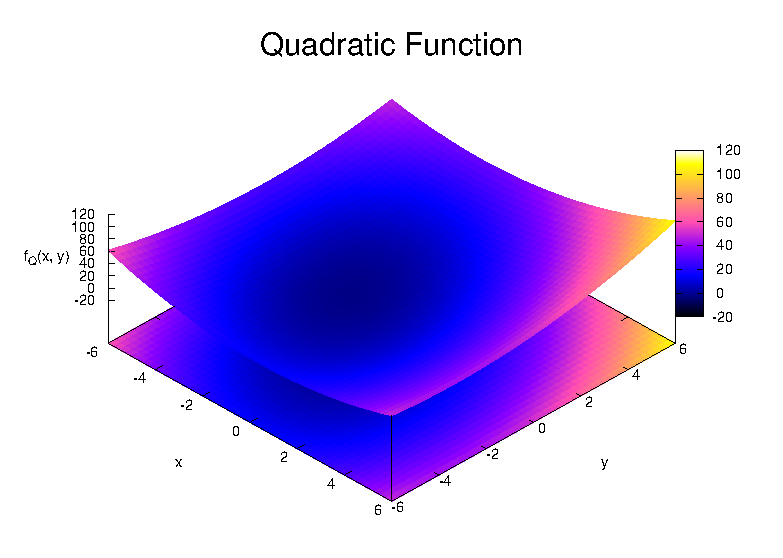
\includegraphics[width=0.9\textwidth]{./images/quadratic_function}
\caption{Note the basin (dark region in the middle)}
\end{minipage}
\hfill
\begin{minipage}{0.45\linewidth}
\centering
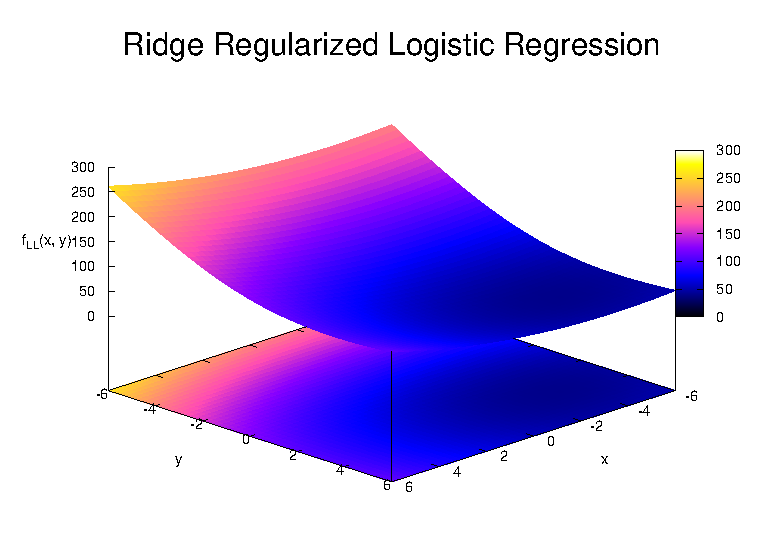
\includegraphics[width=0.9\textwidth]{./images/ridge_regularized_logistic_regression}
\caption{Note the basin (slightly darker region near \((-4, 4)\))}
\end{minipage}
\end{figure}

\begin{figure}[H]
\begin{minipage}{0.45\linewidth}
\centering
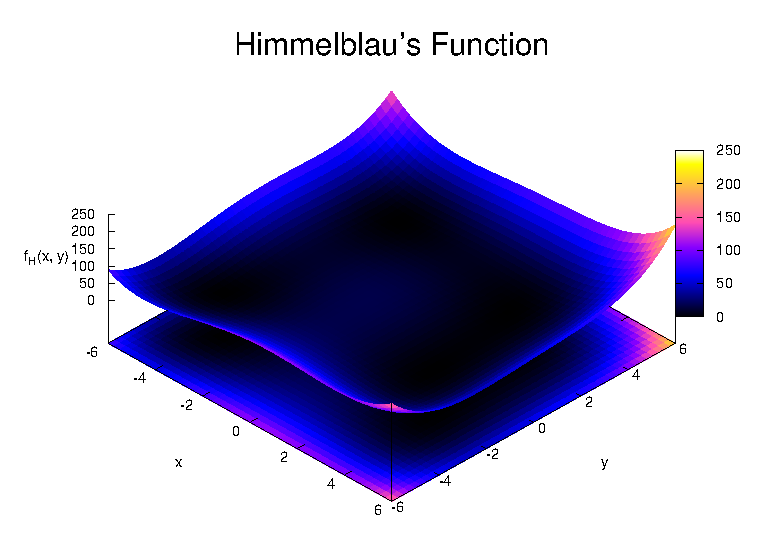
\includegraphics[width=0.9\textwidth]{./images/himmelblaus_function}
\caption{Note the 4 basins and a plateau approximately in the middle of them}
\end{minipage}
\hfill
\begin{minipage}{0.45\linewidth}
\centering
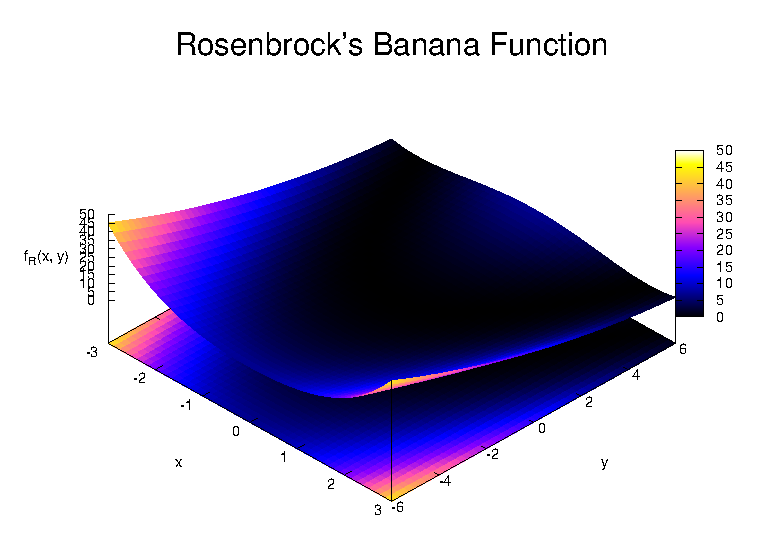
\includegraphics[width=0.9\textwidth]{./images/rosenbrock_banana_function}
\caption{Note the valley (dark parabolic structure)}
\end{minipage}
\end{figure}

Gradient Descent was the algorithm used to find attain the closest minimum from the point of initialization. The reason \textit{closest minimum} is explicitly mentioned is because of the existence of multiple minima in the Himmelblaus function, and the dynamics of Gradient Descent dictate that the result of the algorithm will lie at the closest basin of attraction.
\(\newline\)

We are going to evaluate the performance of different learning rate settings for the static initialization at \((2,3)\) by considering the different in the function values at the optimal and last update i.e., \(1000^{th}\) iteration. The optimal values calculated analytically (or using the Newton-Raphson method for \(f_{LL}(x, y)\)) are as follows:
\begin{center}
\begin{tabular}{|c|c|c|}
\hline
Function & Optimal Value in domain & Attained at \\
\hline
Quadratic Function & \(0.0\) & \((-0.64, -1.12)\)\\
\hline
Ridge Regularized Logistic Regression & \(\approx 40.4012\) & \((-3.3742, 3.5787)\)\\
\hline 
Himmelblaus Function & \(0.0\) & \((3, 2)\)\\
\hline
Rosenbrock's Banana Function & \(0.0\) & \((1, 1)\)\\
\hline
\end{tabular}
\end{center}

The first Gradient Descent method used was Vanilla Gradient Descent with a fixed step size to be chosen from \(\lbrace 0.3, 0.1, 0.01 \rbrace\). The point of initializations were one fixed point -- \((2,3)\) for all functions and two other points chosen randomly from the domain in consideration of the functions. My implementation chooses these points from a uniform distribution over the domain of the functions. The below table shows the difference \(f(\mathbf{x}^{(1000)}) - f(\mathbf{x}^{*})\) for initialization at \((2,3)\).
\(\newline\)

\begin{table}[H]
\centering
\begin{tabular}{|c|c|c|c|}
\hline
\(\eta \rightarrow\) & 0.3 & 0.1 & 0.01 \\
\hline
\(f_{Q}(x, y)\) & 0 & 0 & 0\\
\hline
\(f_{LL}(x, y)\) & 0 & 0 & 0\\
\hline
\(f_{H}(x, y)\) & 1.769 & 0 & 0 \\
\hline
\(f_{R}(x, y)\) & 0.00092 & 0.00106 & 0.00112 \\
\hline
\end{tabular}
\caption{\(f(\mathbf{x}^{(1000)}) - f(\mathbf{x}^{*})\) for Fixed Step Size}
\end{table}

From the above table it can be seen that for any setting of learning rate from the given values, the algorithm converges to the minimum for the convex functions: \(f_{Q}\) and \(f_{LL}\). This is natural from what we have learnt that gradient descent will eventually converge to the minimum for convex functions. In \(f_{H}\), convergence was seen for the step size being set to \(0.1\) and \(0.01\), but there was an oscillation observed in \(0.3\), hence the point got pushed away from the minimum. 

\begin{figure}[H]
\begin{minipage}{0.32\linewidth}
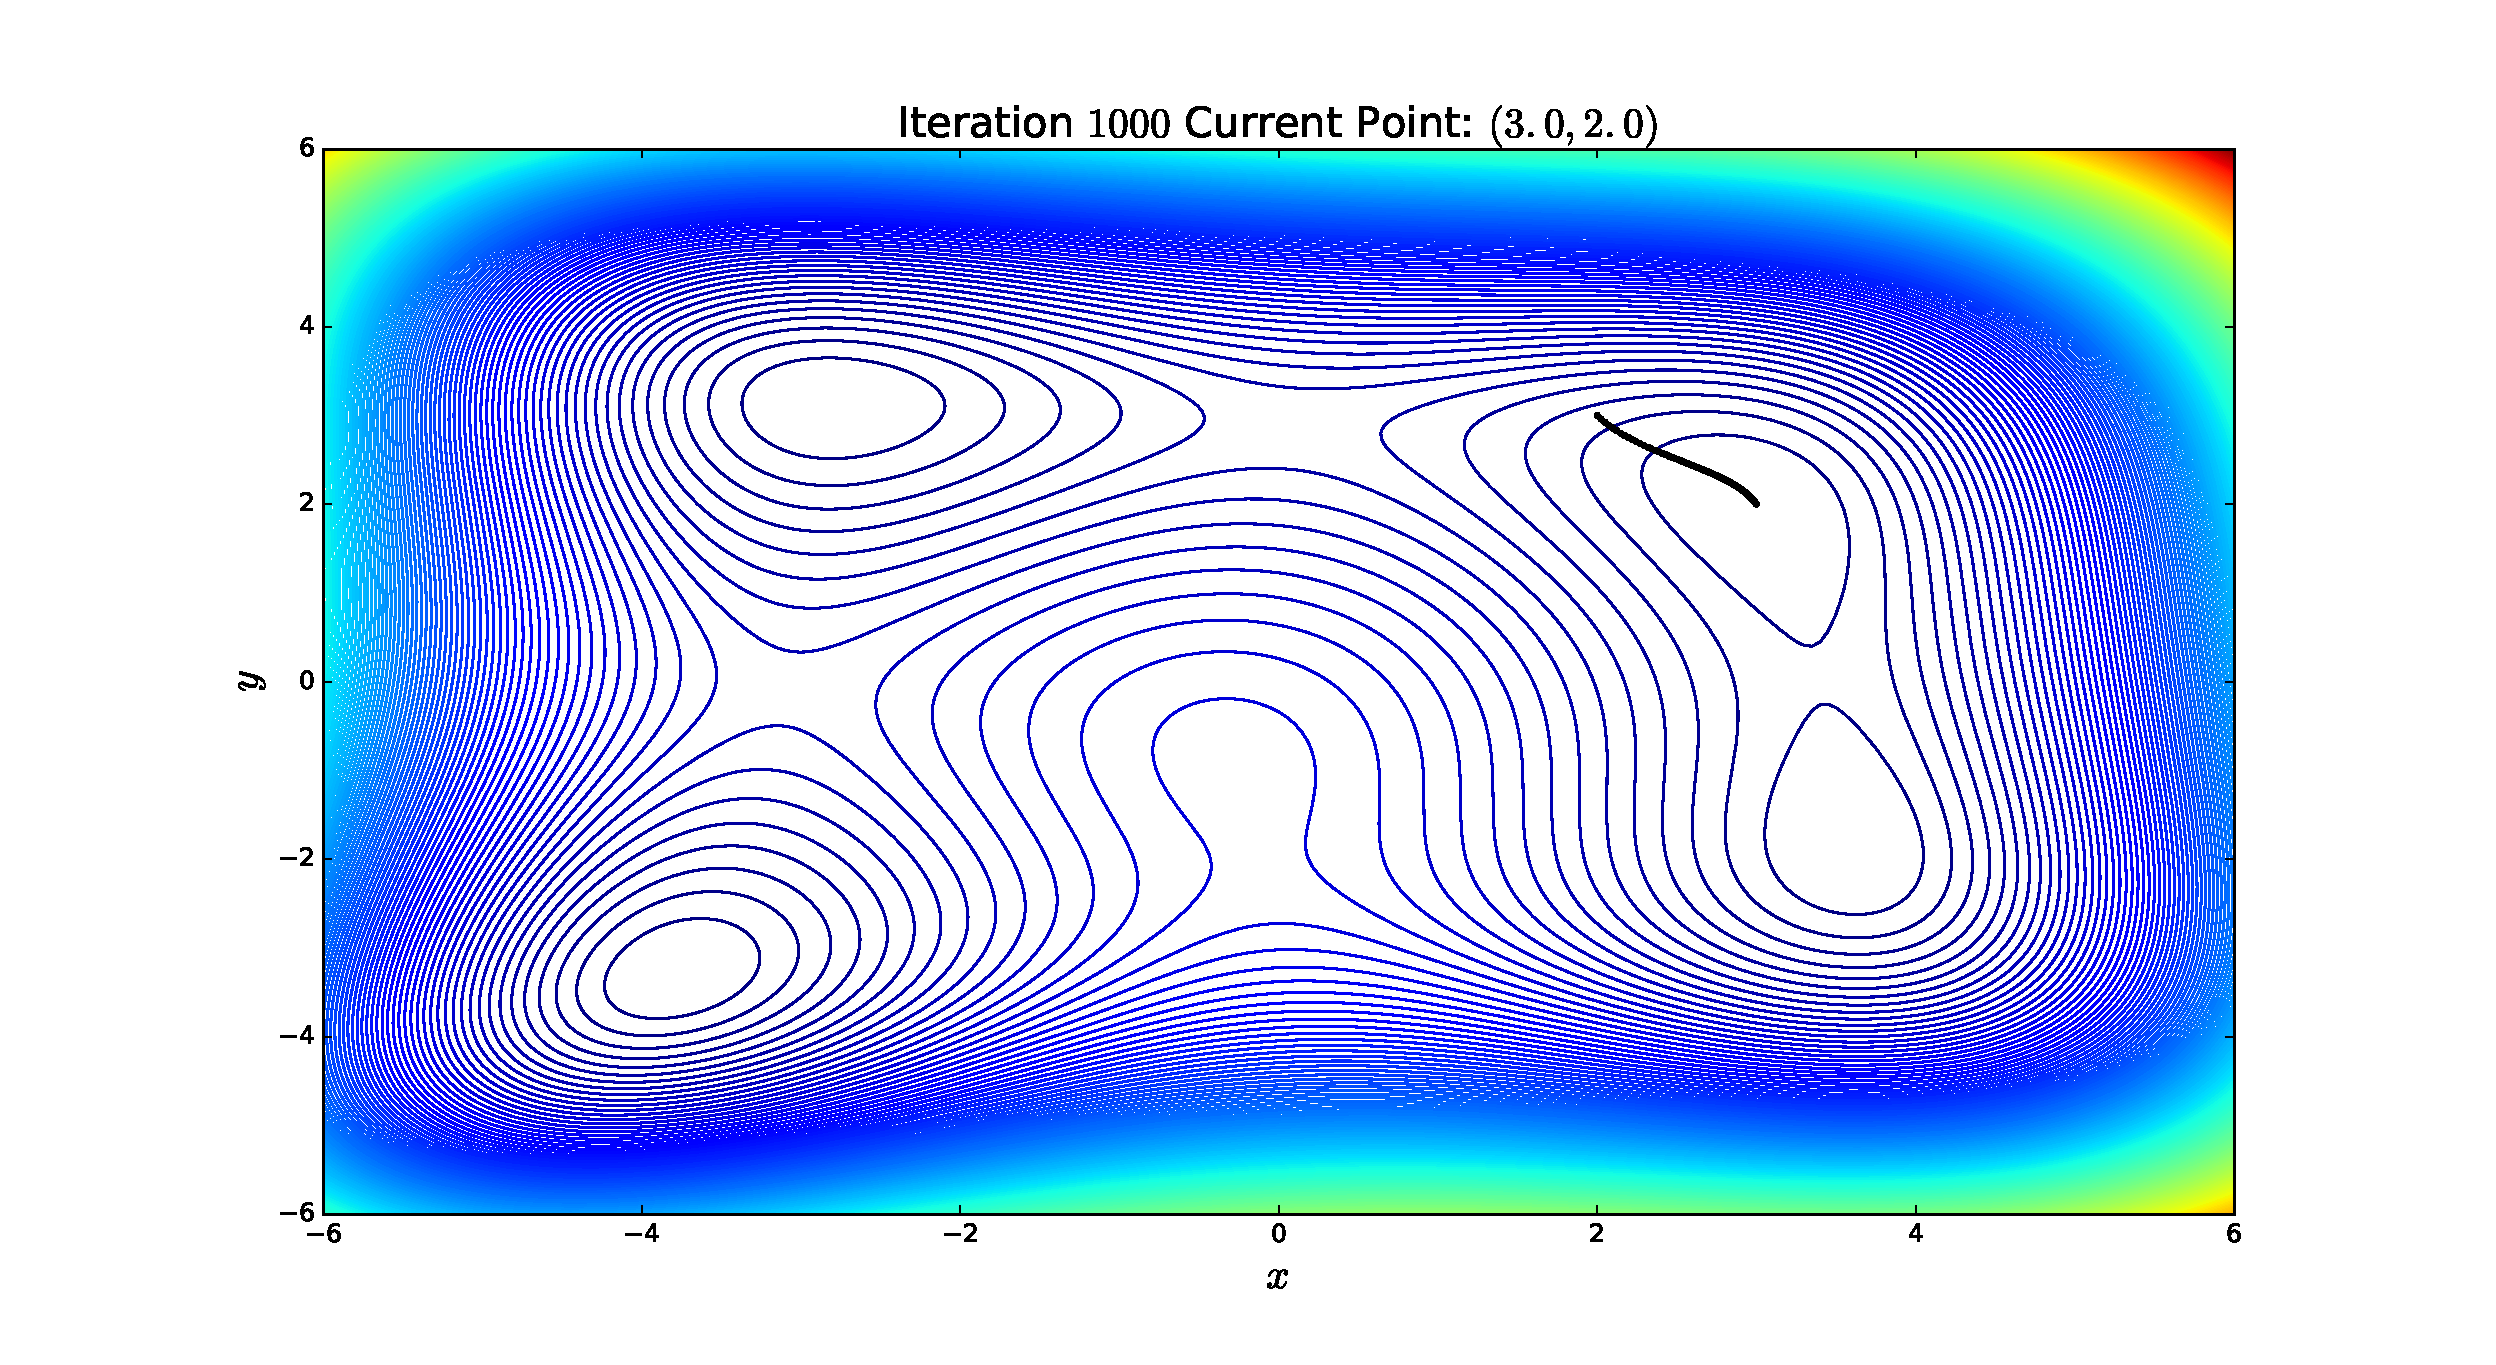
\includegraphics[width=0.9\textwidth]{./images/himmelblau_0_01.eps}
\caption{\(f_{H}(x, y) \rightarrow \eta\) = 0.01}
\end{minipage}
\hfill
\begin{minipage}{0.32\linewidth}
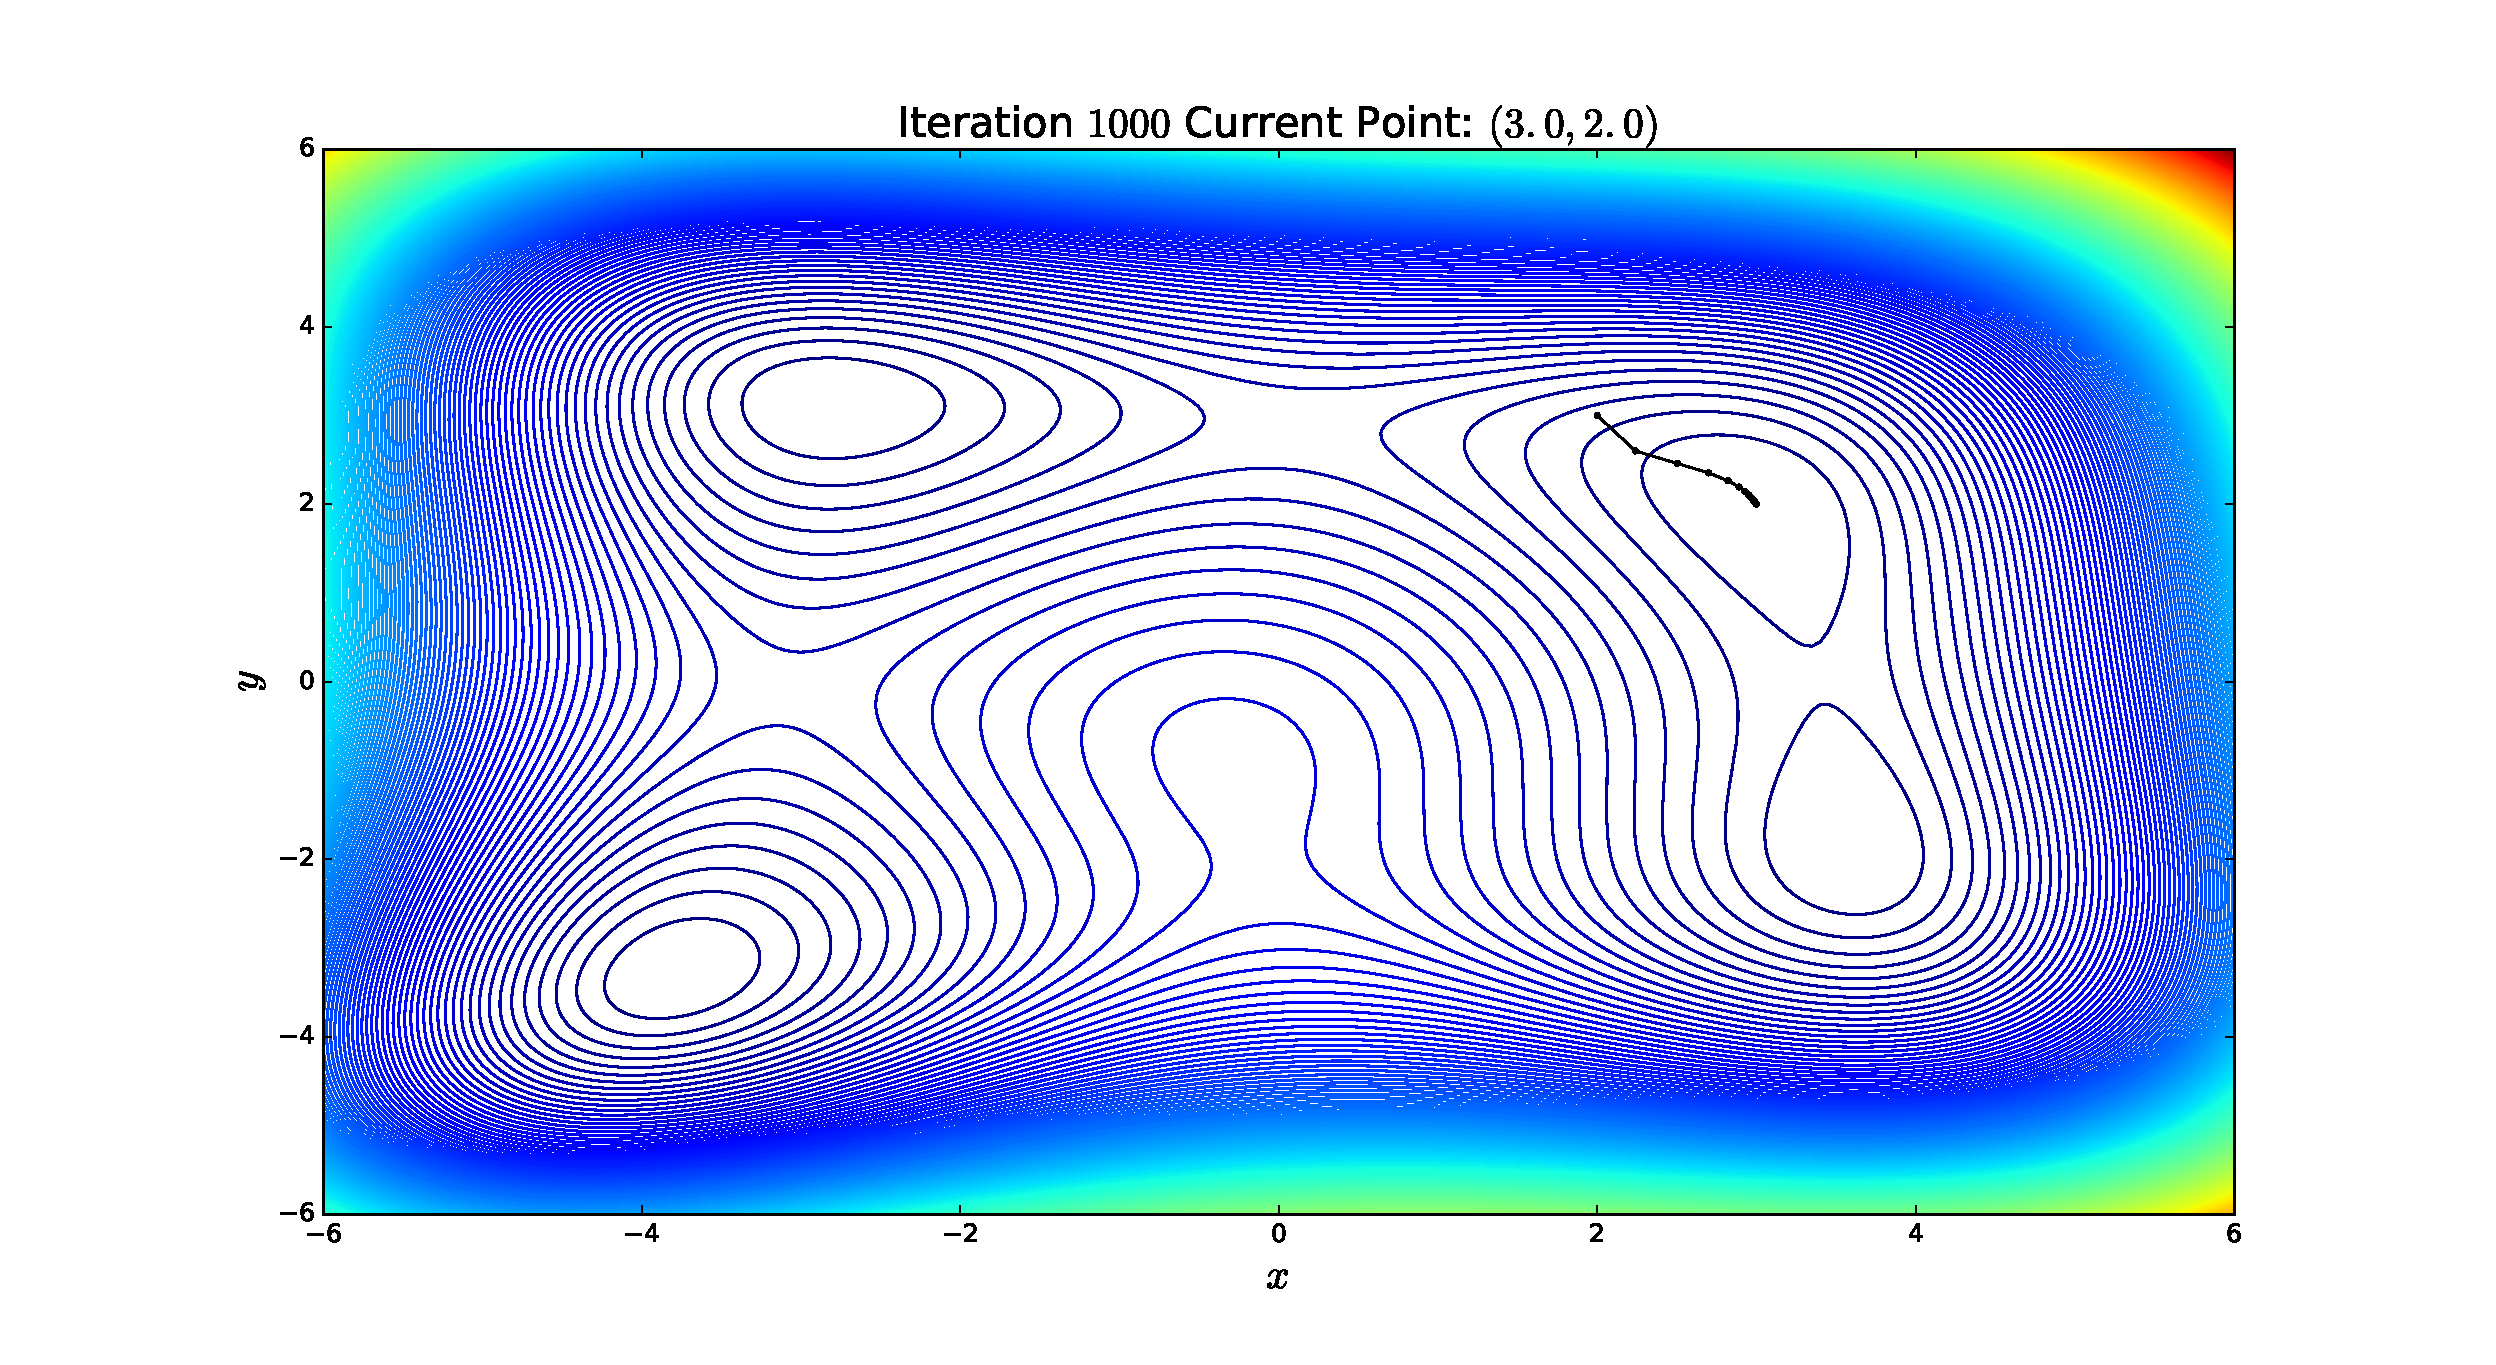
\includegraphics[width=0.9\textwidth]{./images/himmelblau_0_1.eps}
\caption{\(f_{H}(x, y) \rightarrow \eta\) = 0.1}
\end{minipage}
\hfill
\begin{minipage}{0.32\linewidth}
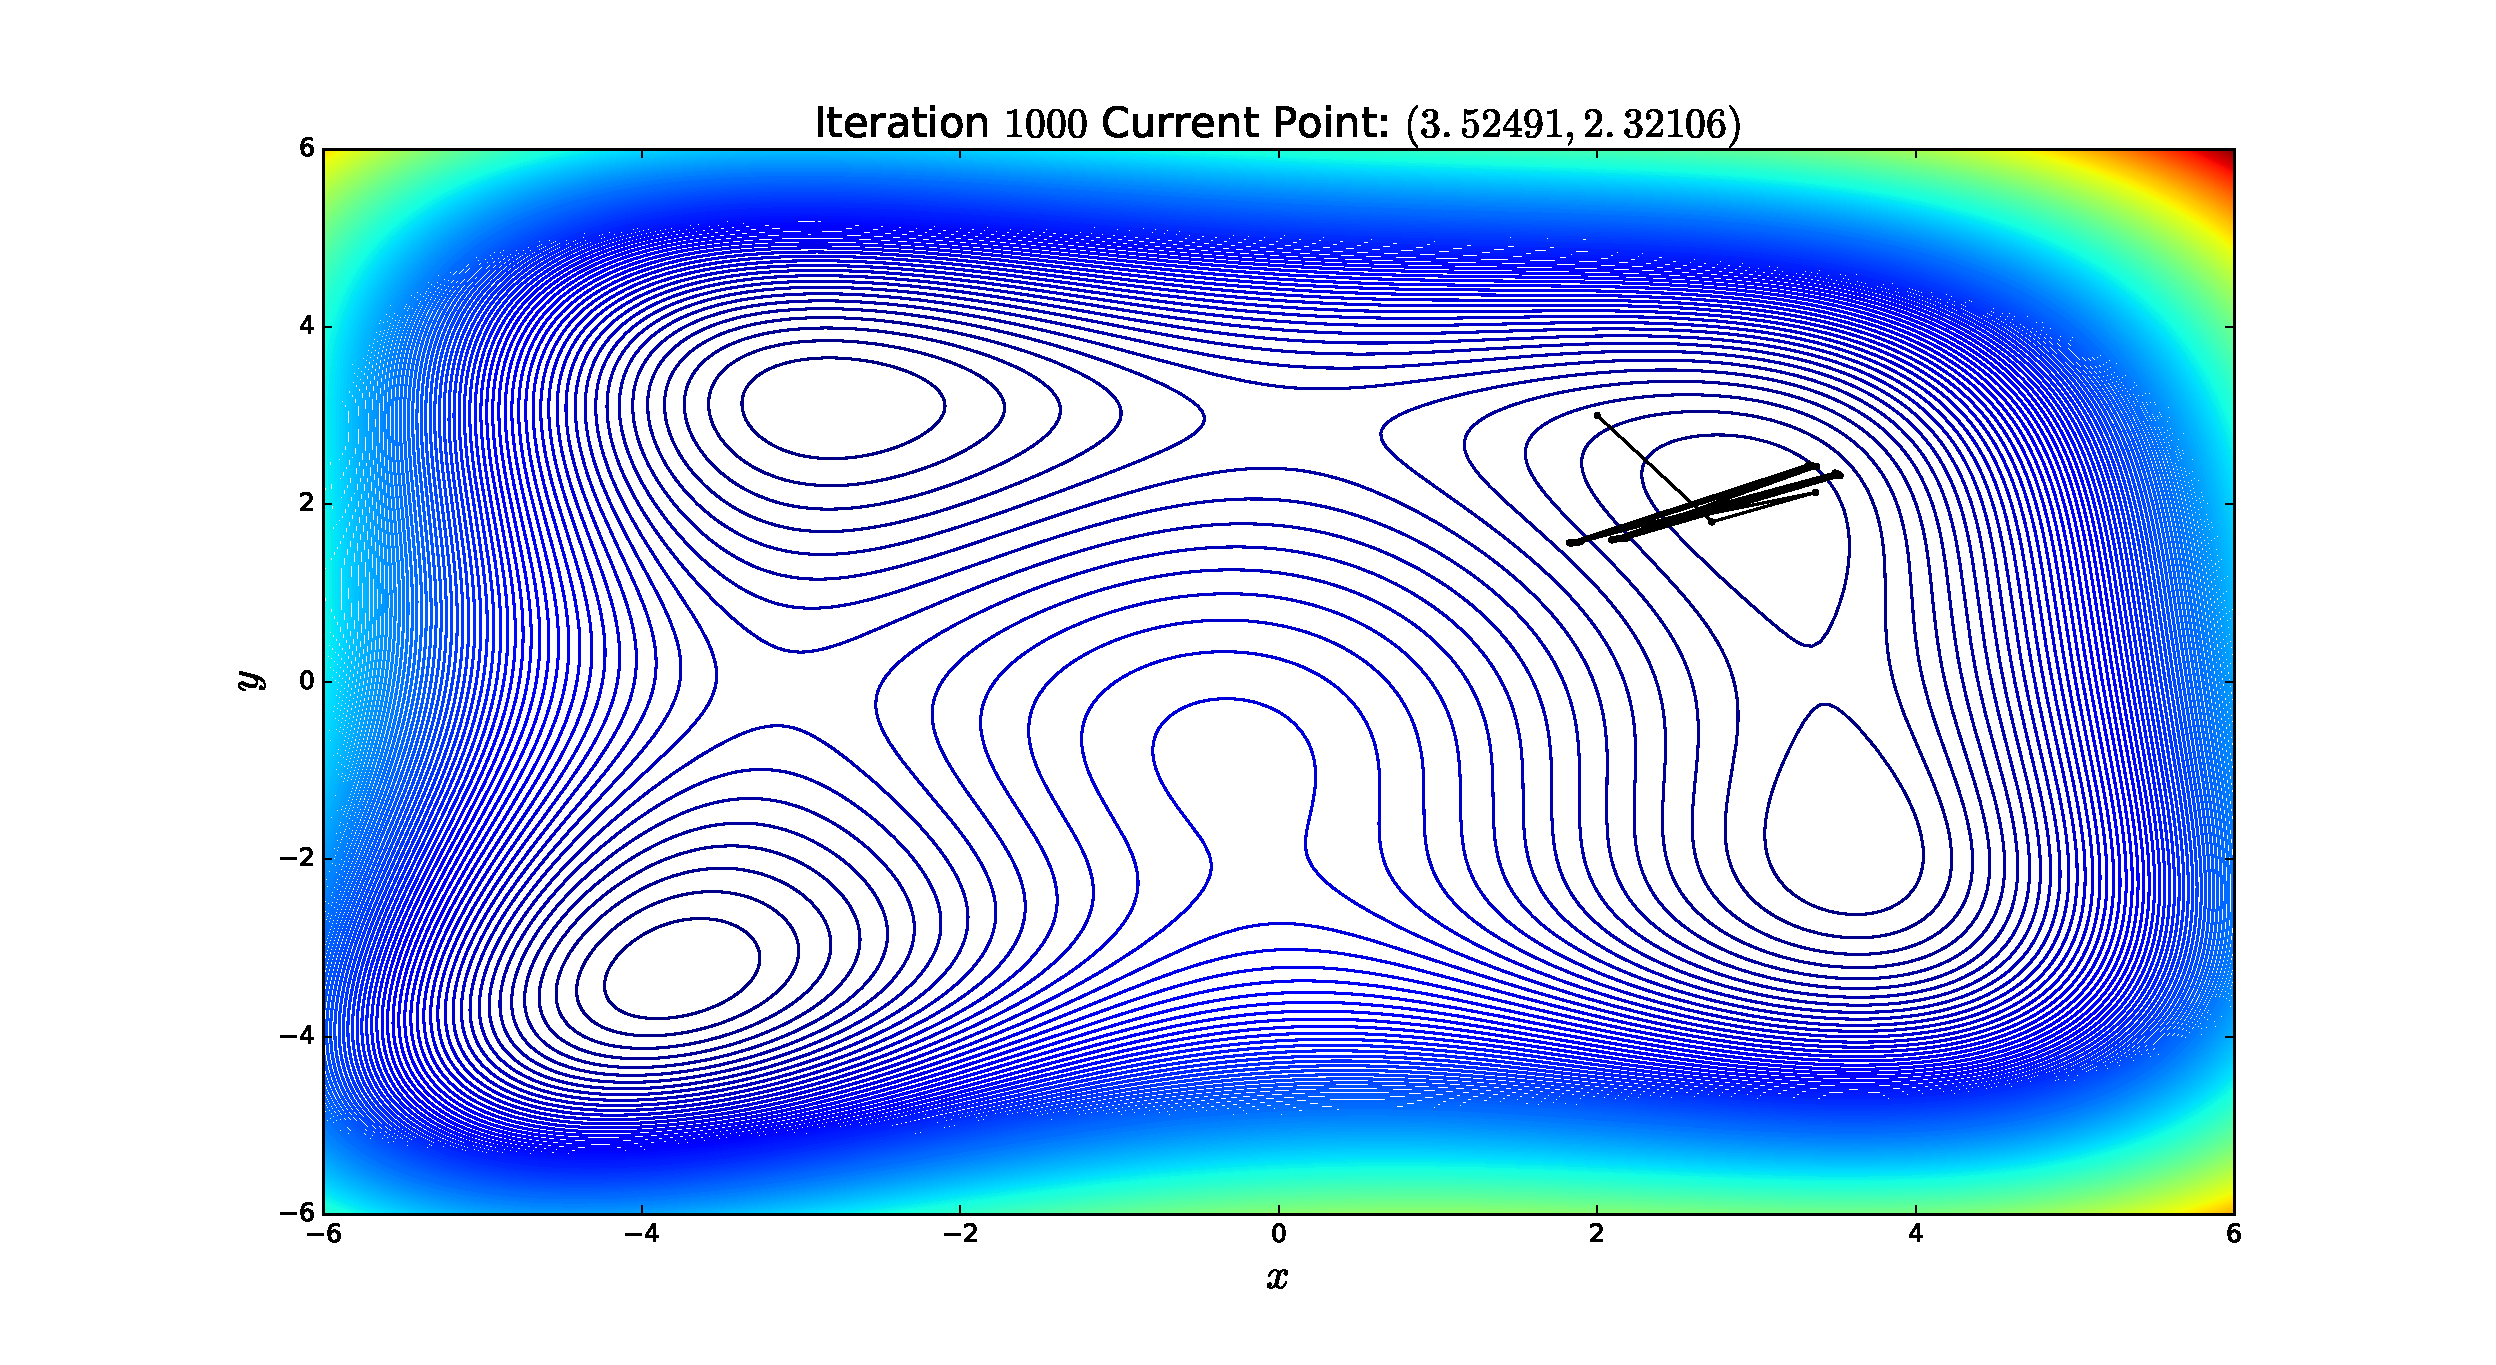
\includegraphics[width=0.9\textwidth]{./images/himmelblau_0_3.eps}
\caption{\(f_{H}(x, y) \rightarrow \eta\) = 0.3}
\end{minipage}
\end{figure}
In the case of \(f_{R}\), the valley like structure makes the gradient updates slower and slower and hence none of the settings make it to the minimum.
\(\newline\)

The next Gradient Descent method used was Backtracking Line Search with Gradient Descent. Here we consider the approximation:
\begin{equation*}
f(\mathbf{x} + t\nabla f(\mathbf{x})) \approx f(\mathbf{x}) - t\alpha ||\nabla f(\mathbf{x})||^{2}_{2}
\end{equation*}
\(\newline\)

The update step for \(t\) is \(t := \beta t\). \(\alpha = 0.5\) and \(\beta = 0.5\) is our settings. Below are the value of \(f(\mathbf{x}^{(1000)}) - f(\mathbf{x}^{*})\) for initialization at \((2,3)\).
\(\newline\)

\begin{table}[H]
\centering
\begin{tabular}{|c|c|c|c|}
\hline
\(f_{Q}(x, y)\) & \(f_{LL}(x, y)\) & \(f_{H}(x, y)\) & \(f_{R}(x, y)\) \\
\hline
0 & 0 & 0 & 0.00078 \\
\hline
\end{tabular}
\caption{\(f(\mathbf{x}^{(1000)}) - f(\mathbf{x}^{*})\) for Backtracking Line Search}
\end{table}

This shows the effectiveness of backtracking line search based Gradient Descent. It still could not navigate to the minimum in \(f_{R}(x, y)\), that is the nature of the valley. As learnt in class, we can see the effectiveness of backtracking line search here too.
\(\newline\)

The last Gradient Descent method used was an annealing schedule for the learning rate. We set the learning rate to \(\frac{1}{k}\) where \(k\) is the iteration number. Below are the values of \(f(\mathbf{x}^{(1000)}) - f(\mathbf{x}^{*})\) for initialization at \((2, 3)\).

\begin{table}[H]
\centering
\begin{tabular}{|c|c|c|c|}
\hline
\(f_{Q}(x, y)\) & \(f_{LL}(x, y)\) & \(f_{H}(x, y)\) & \(f_{R}(x, y)\) \\
\hline
0 & 0 & 0 & 0.00062 \\
\hline
\end{tabular}
\caption{\(f(\mathbf{x}^{(1000)}) - f(\mathbf{x}^{*})\) for Annealing Schedule}
\end{table}

The paths are all affected by the initial high learning rate. In the case of \(f_{Q}\), we jump to the other side of the basin in the first step and then jump back again, and then slowly begin to converge. In the case of \(f_{LL}\), we jump to the other side of the minimum and then to and fro about the minimum and then converge. The most interesting case was in \(f_{H}\). Due to the high learning rate, we end near another local minimum close to \((-3.779, -3.283)\) and infact do not converge at the closest local minimum to the point of initialization, which is \((3, 2)\). In \(f_{R}\), we make a relatively large jump, but still get stuck in the valley. From what we have learnt in class, setting large learning rate initially might not help if our initialization is close to any minimum/basin of attraction. Below are the graphs:

\begin{figure}[H]
\begin{minipage}{0.45\linewidth}
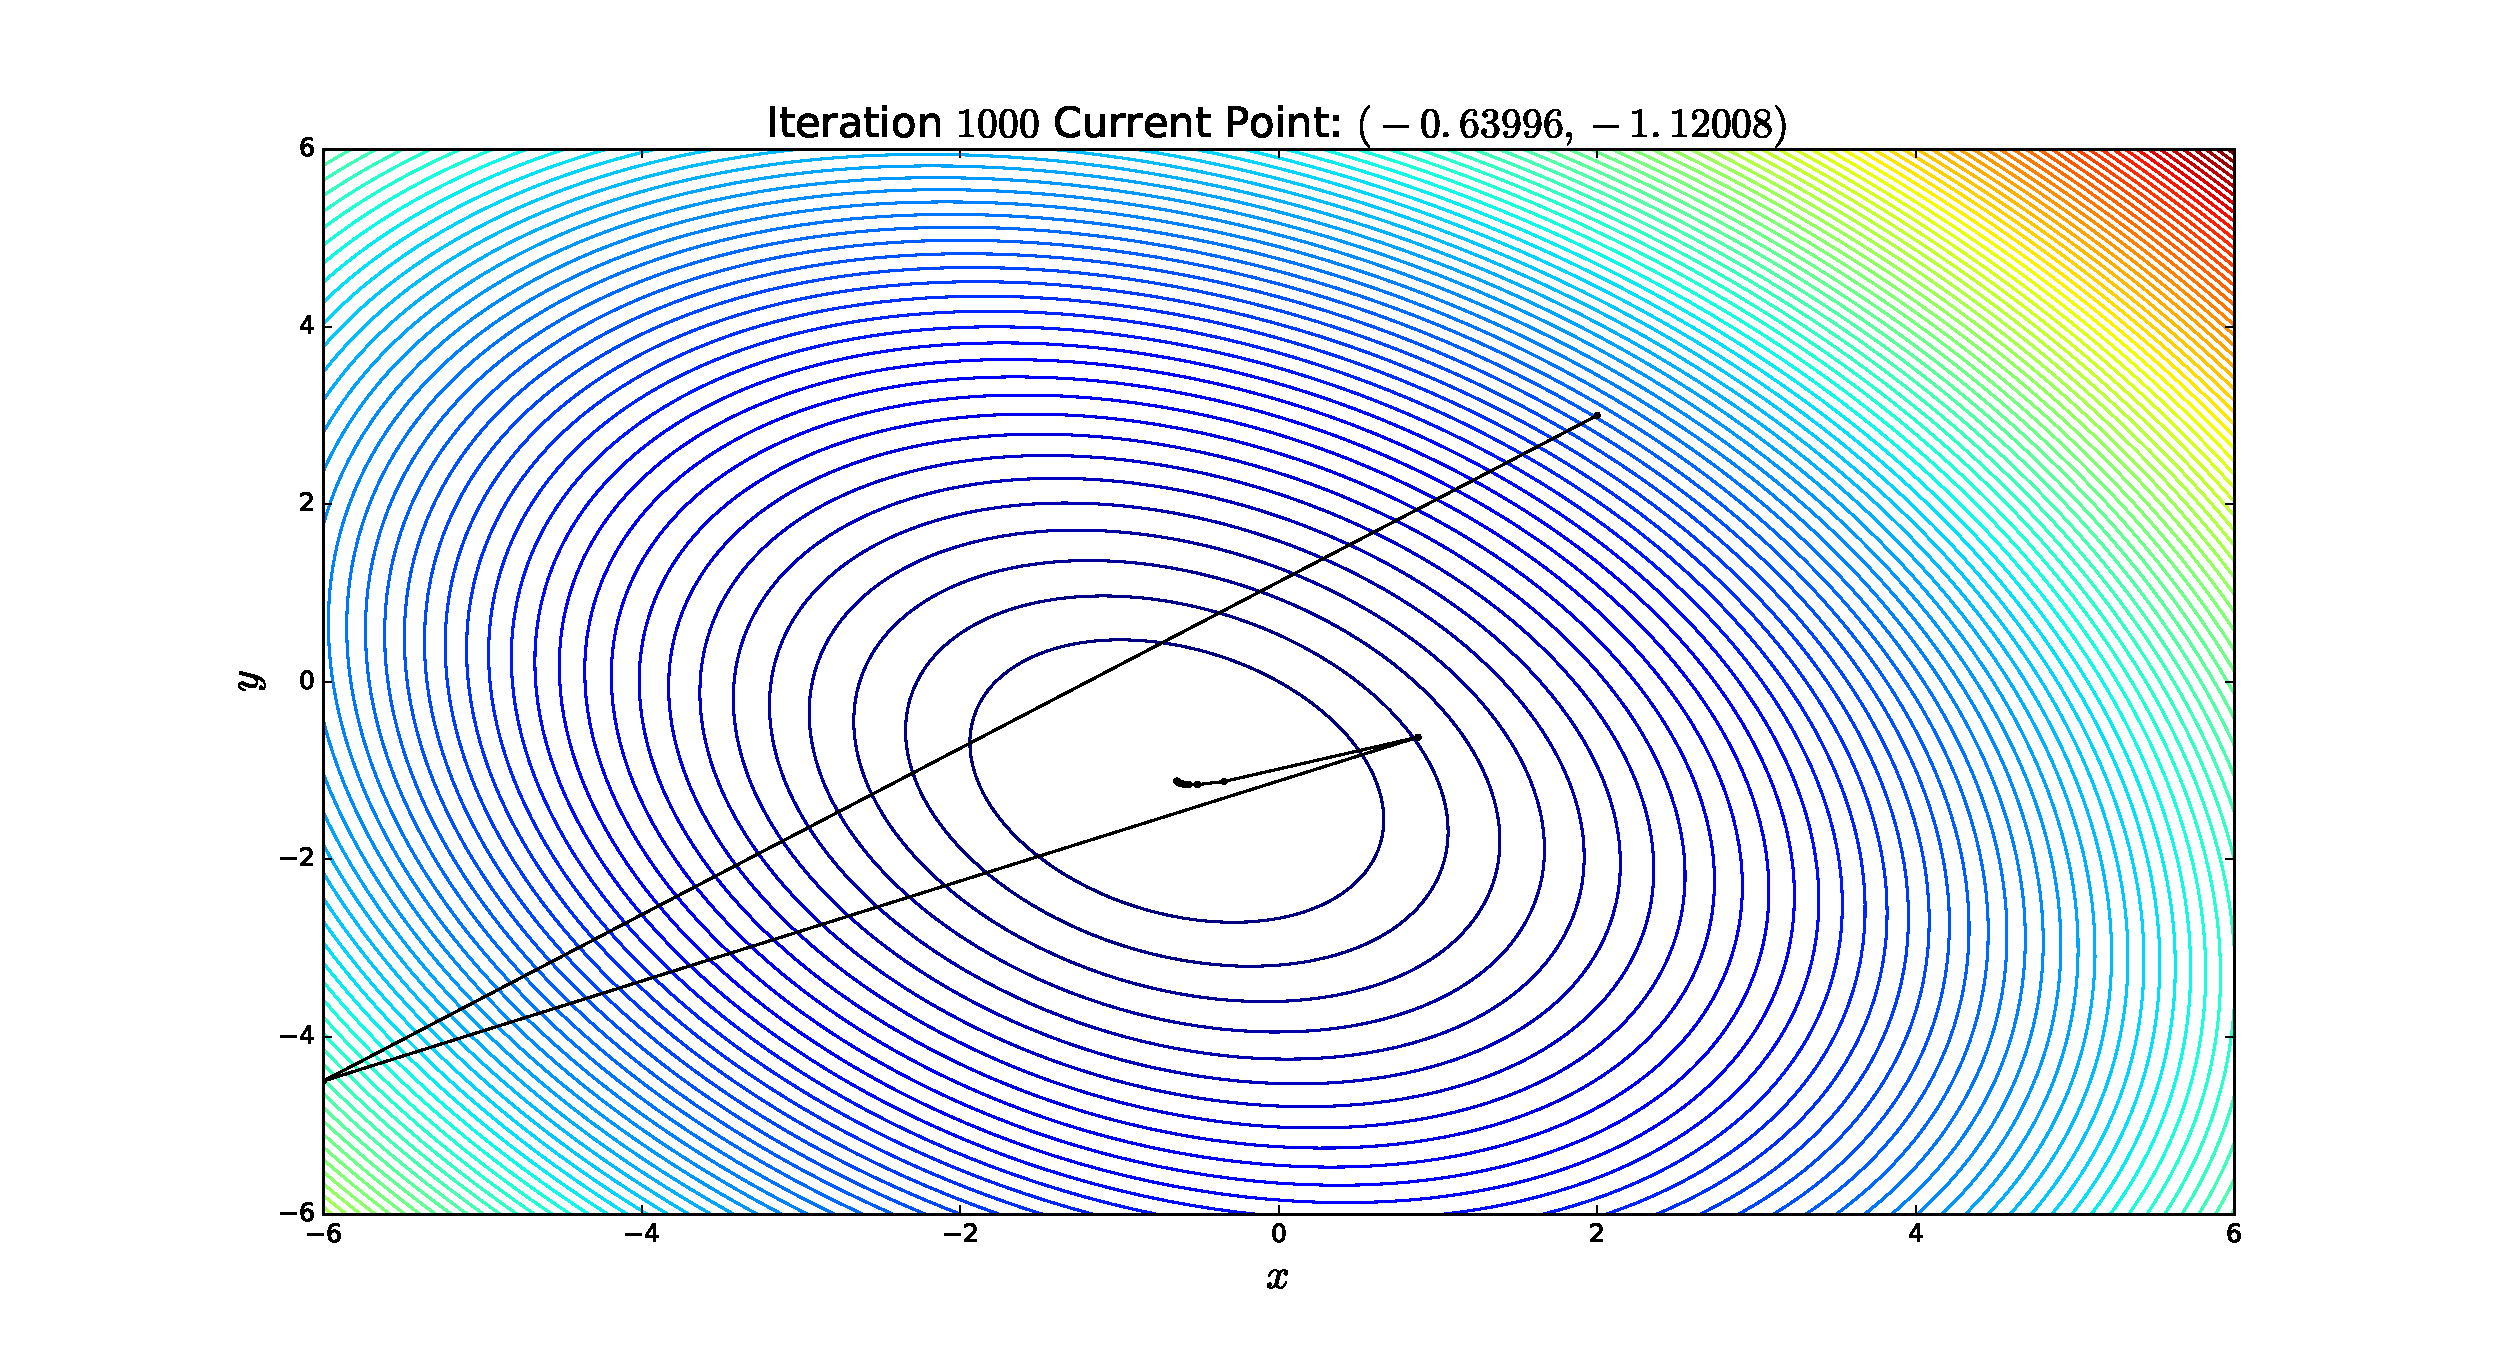
\includegraphics[width=0.9\textwidth]{./images/quad_inv}
\caption{\(f_{Q}\)}
\end{minipage}
\hfill
\begin{minipage}{0.45\linewidth}
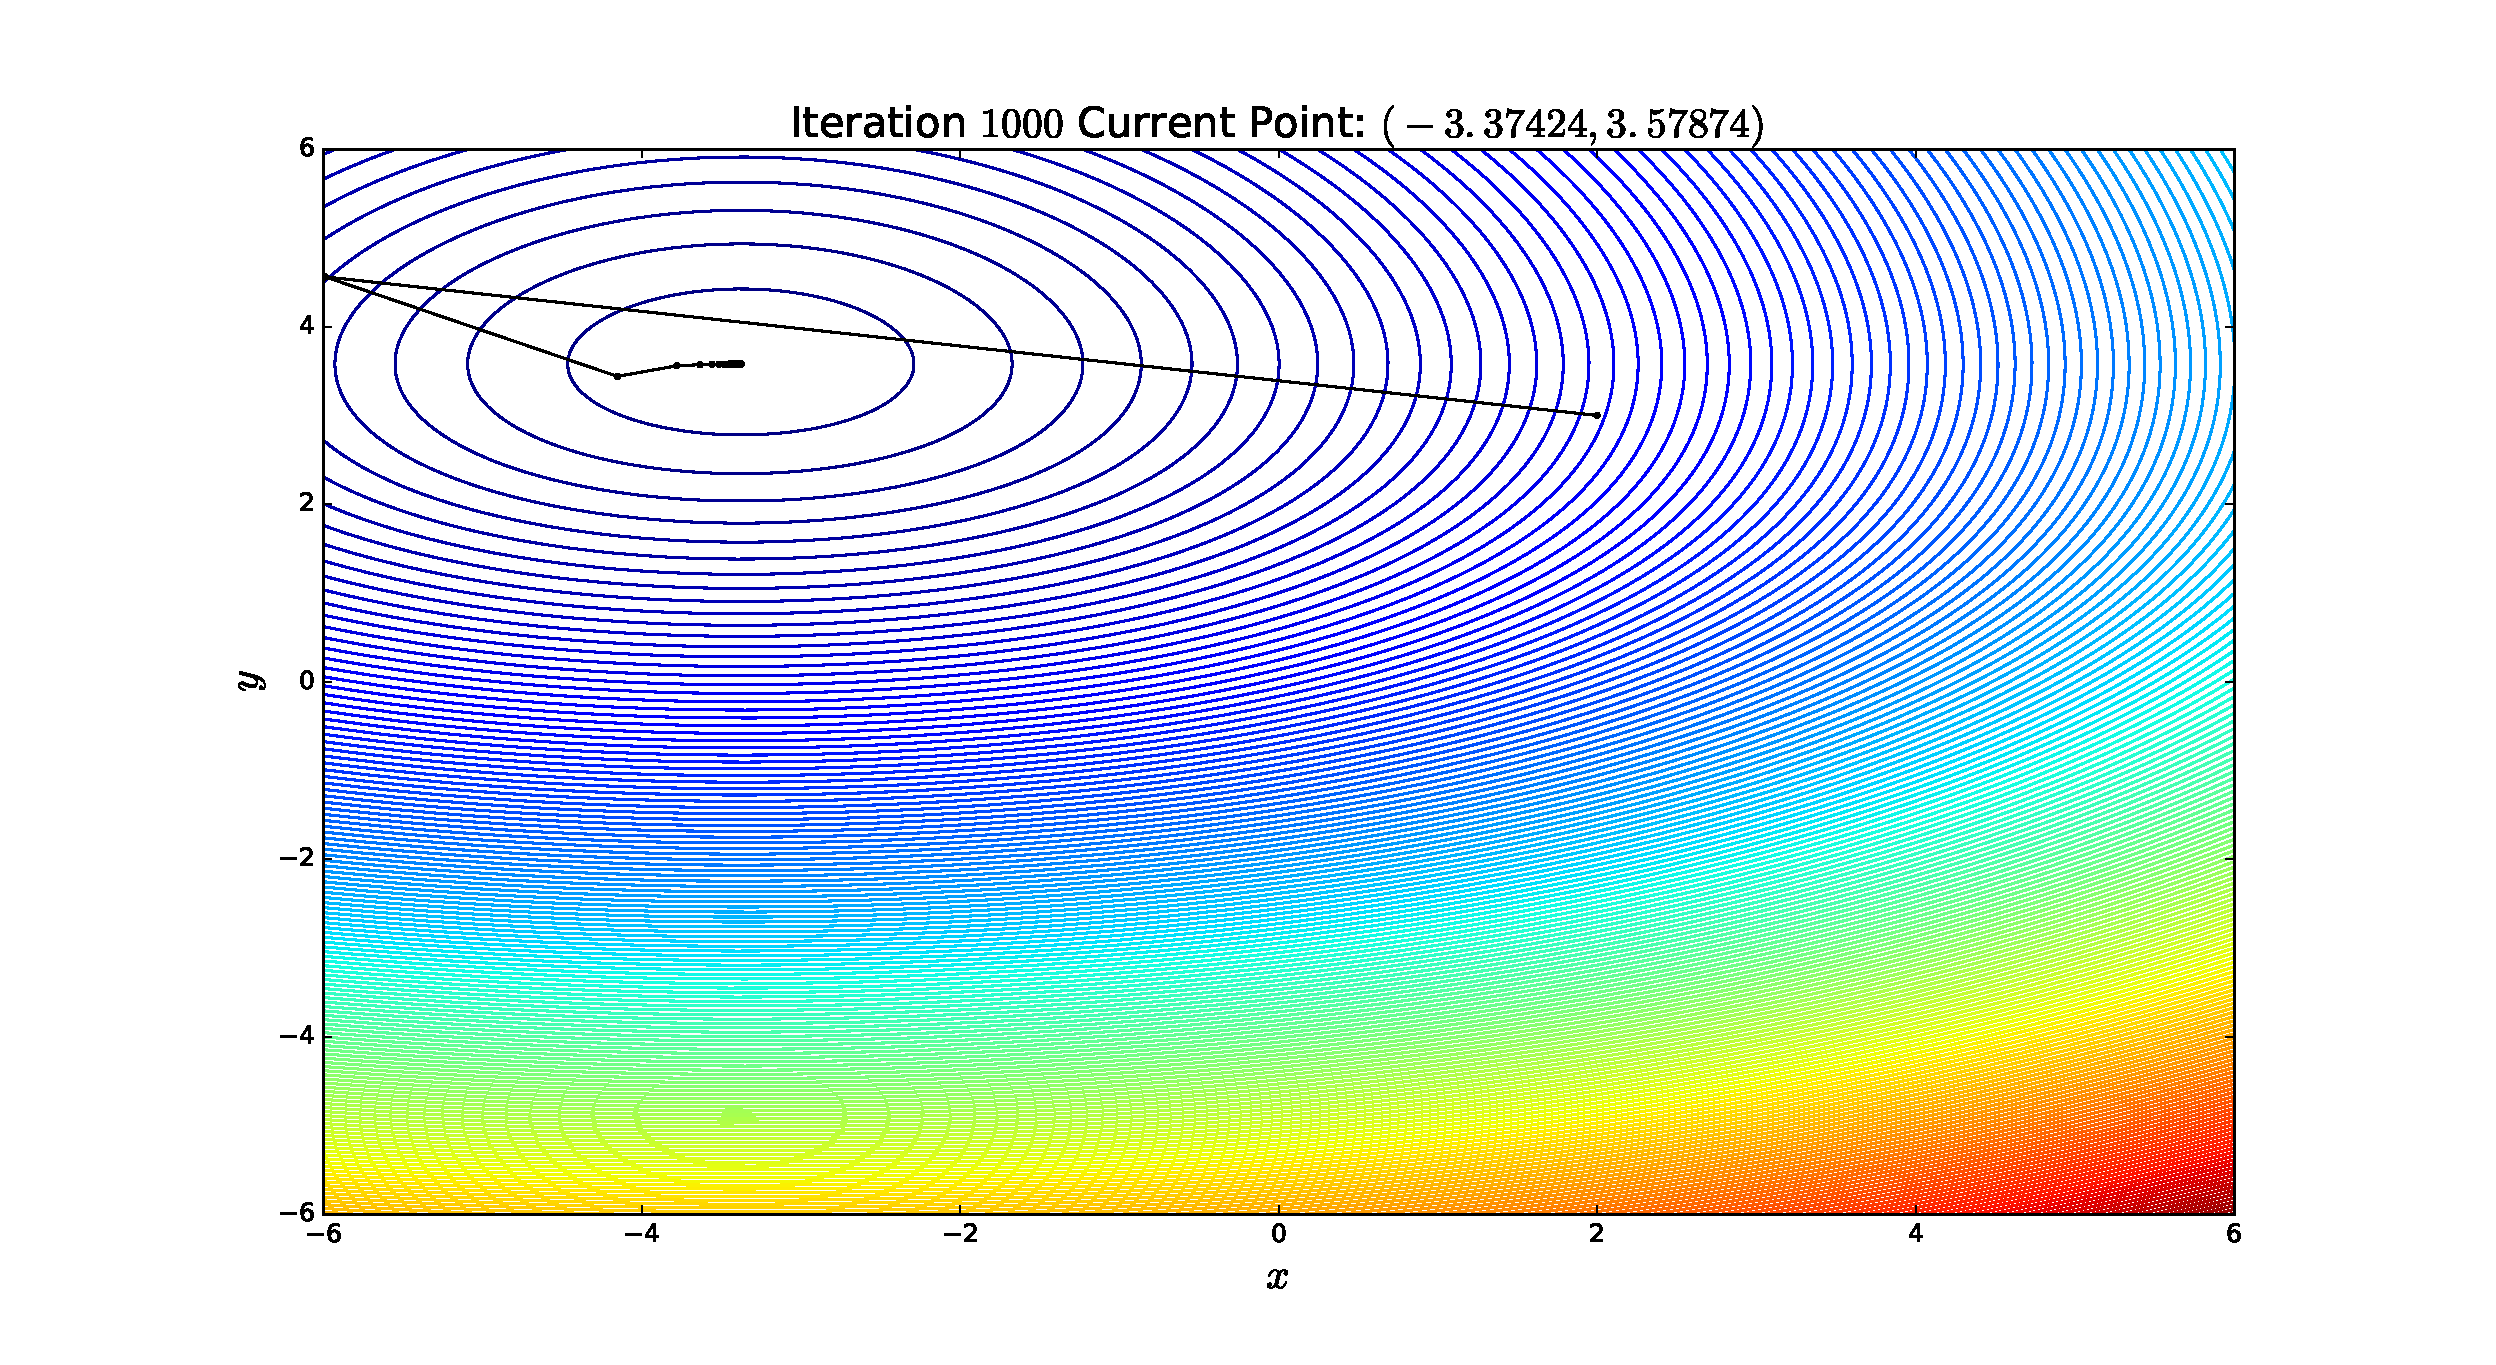
\includegraphics[width=0.9\textwidth]{./images/log_reg_inv}
\caption{\(f_{LL}\)}
\end{minipage}
\end{figure}

\begin{figure}[H]
\begin{minipage}{0.45\linewidth}
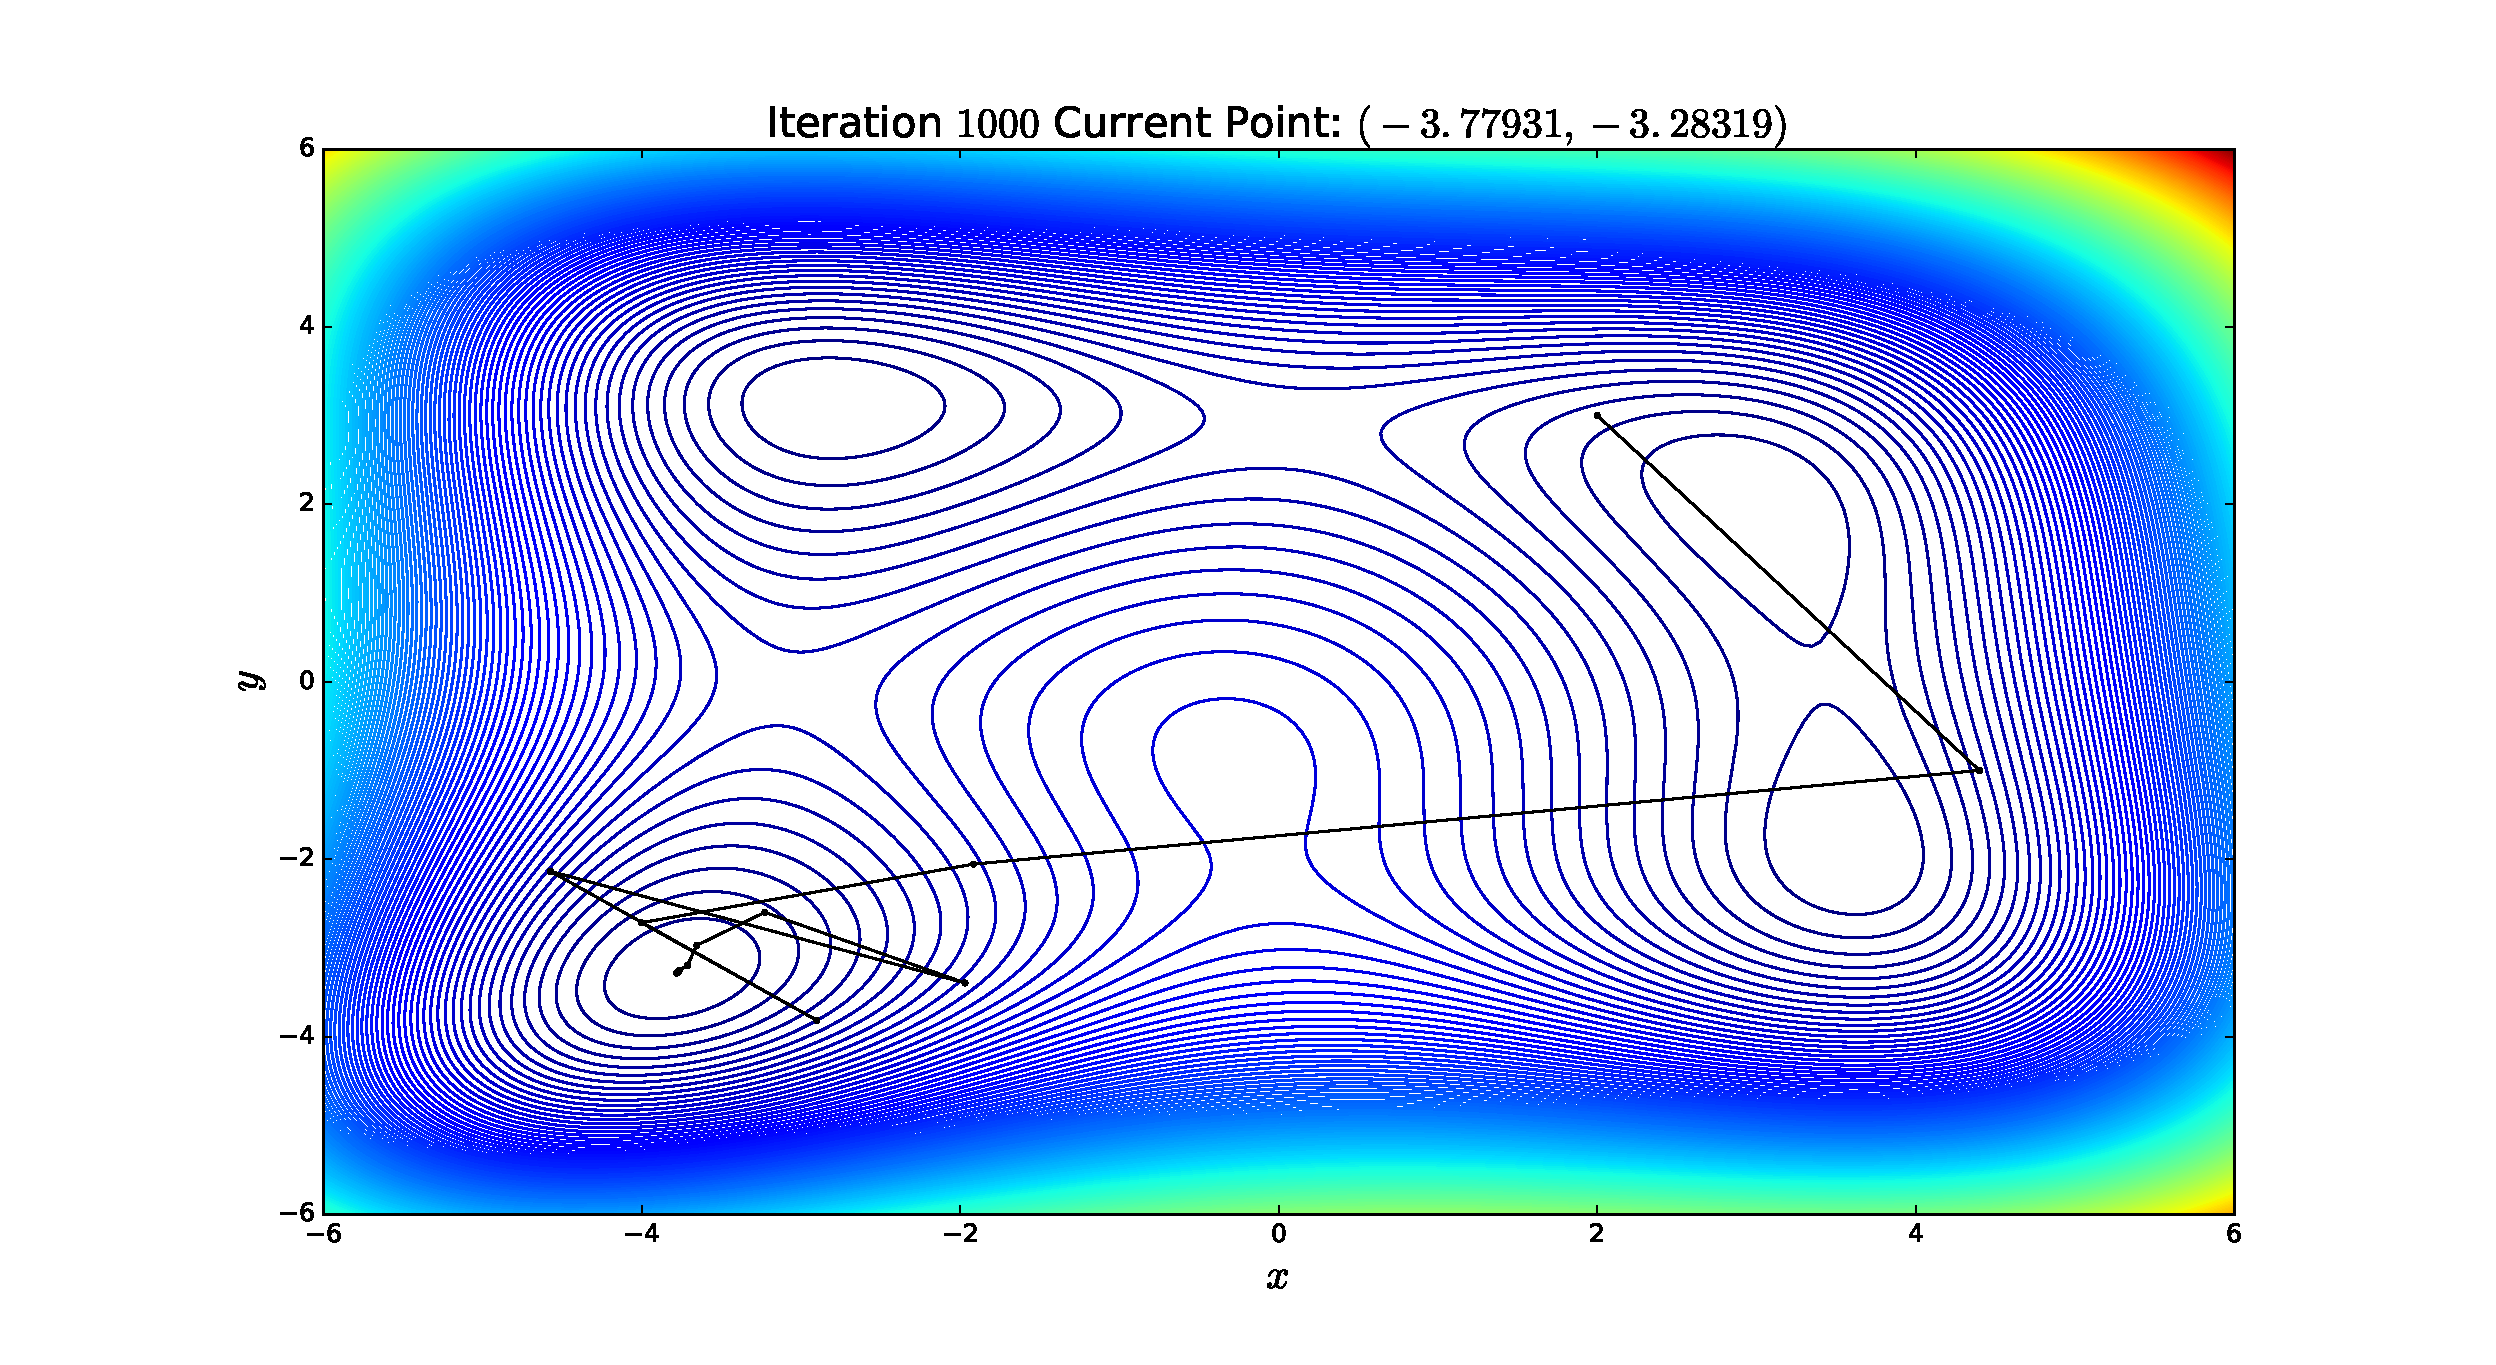
\includegraphics[width=0.9\textwidth]{./images/himmelblau_inv}
\caption{\(f_{H}\)}
\end{minipage}
\hfill
\begin{minipage}{0.45\linewidth}
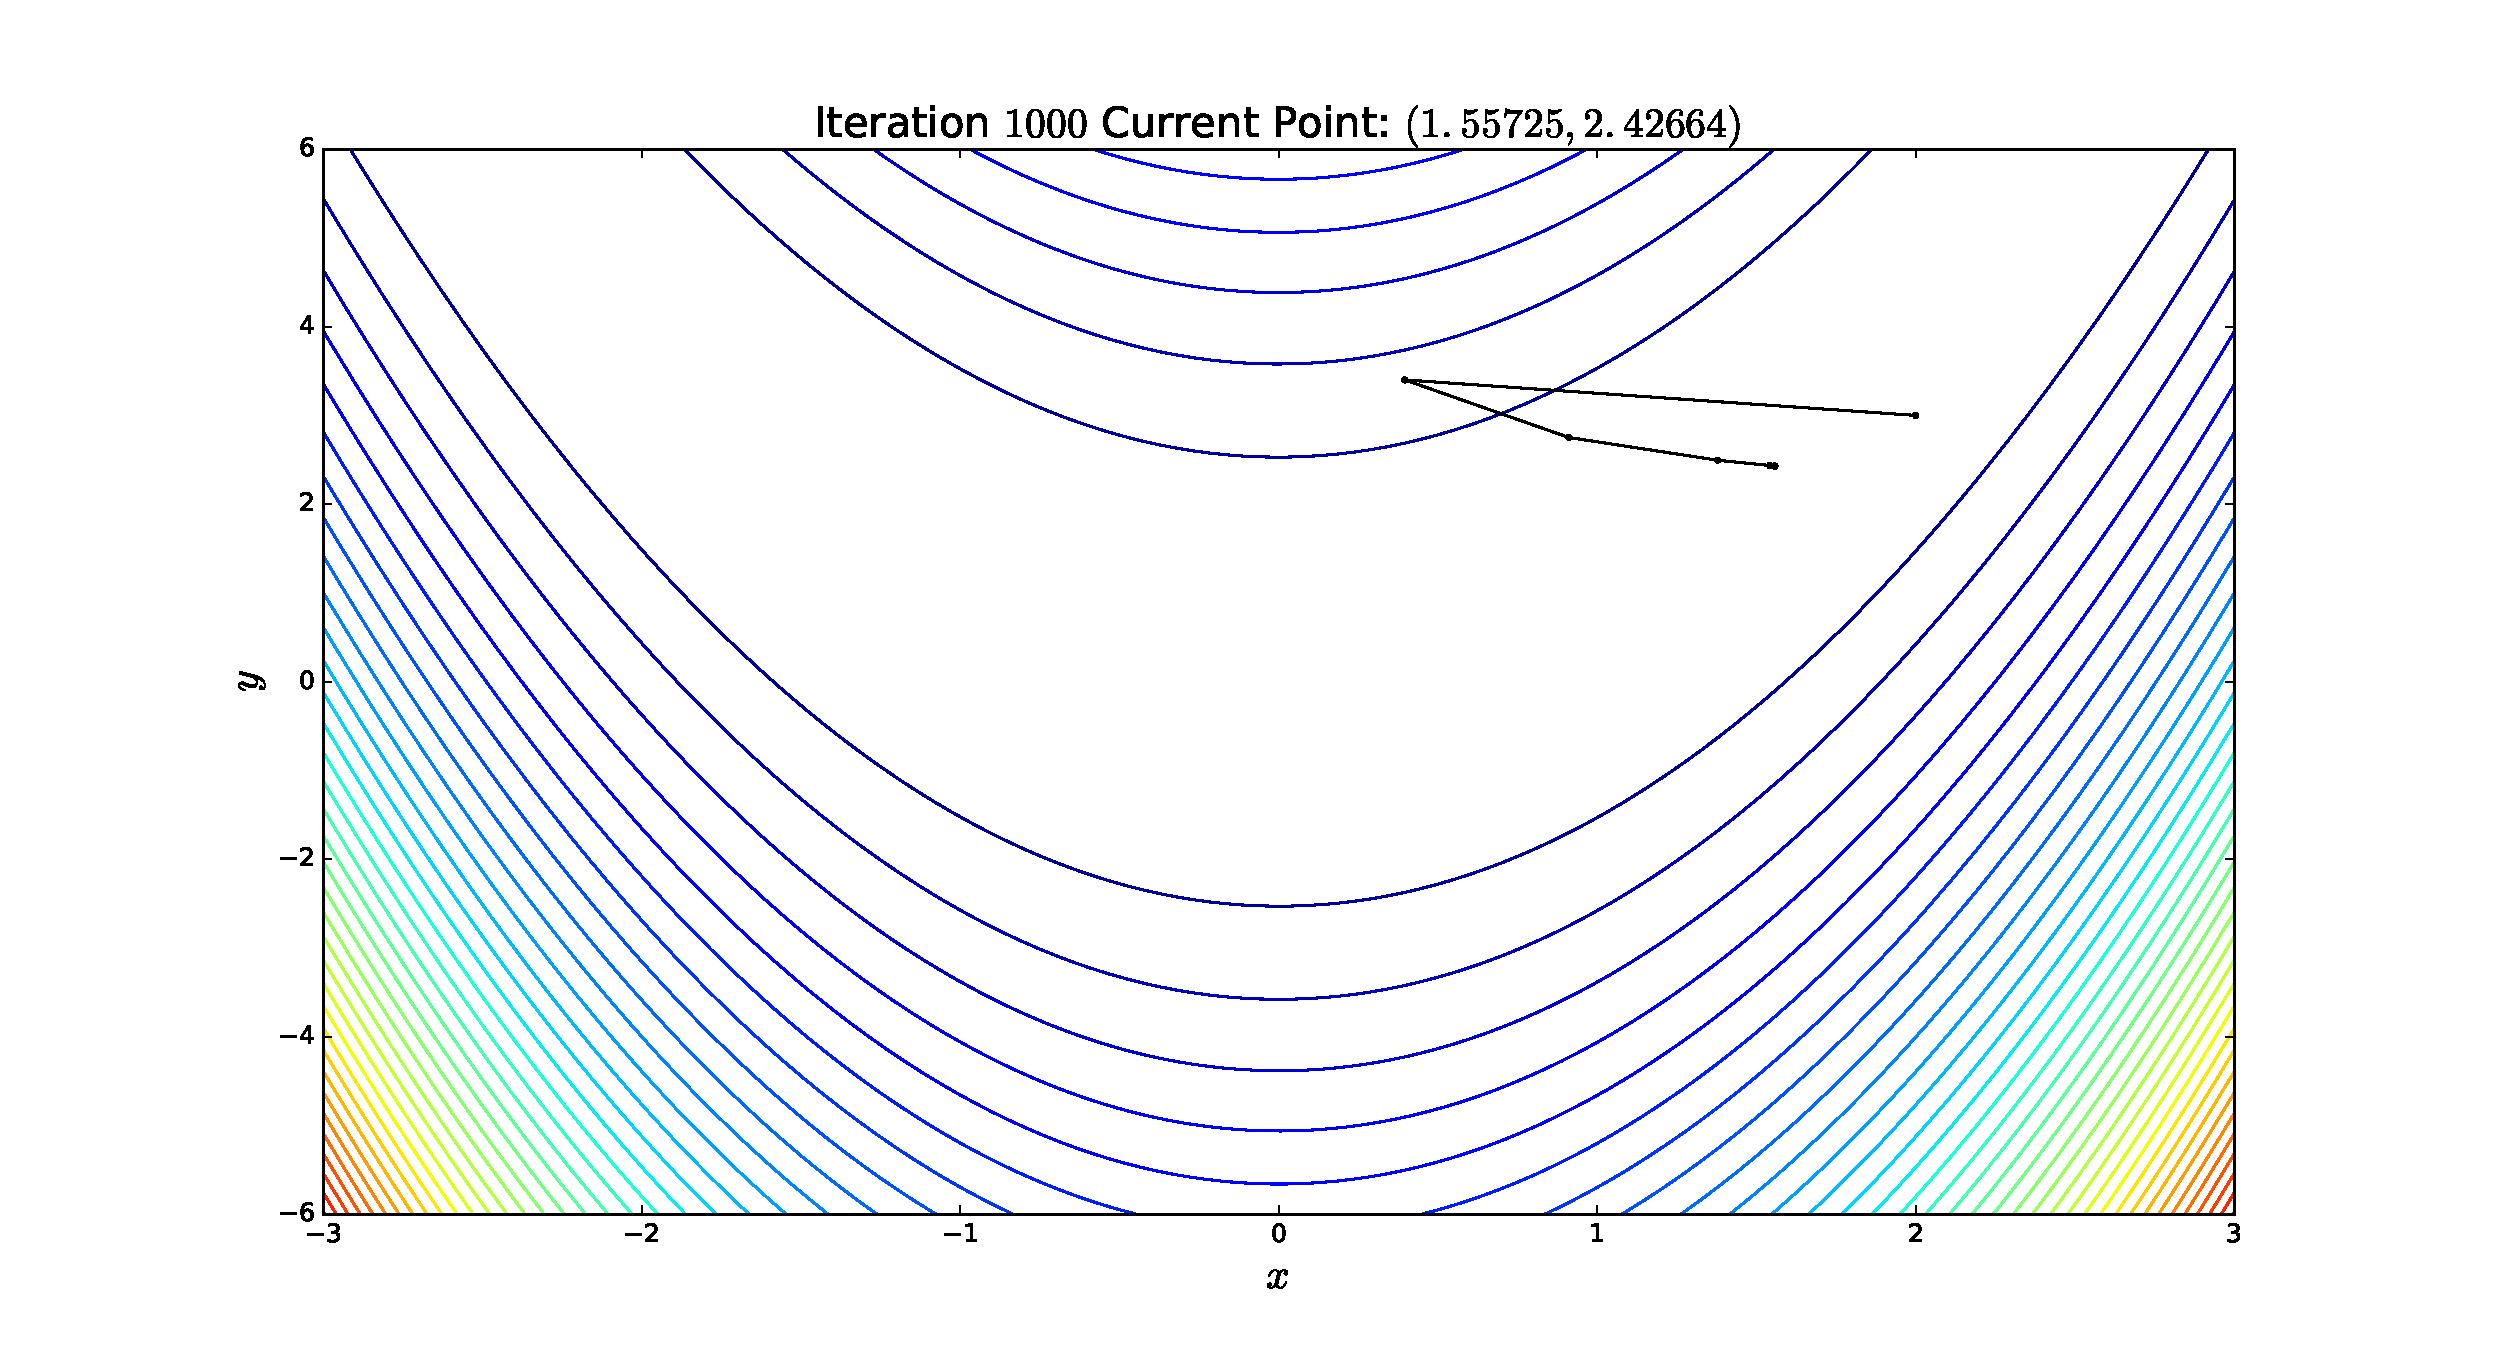
\includegraphics[width=0.9\textwidth]{./images/rosenbrock_inv}
\caption{\(f_{R}\)}
\end{minipage}
\end{figure}

From Yann LeCun's paper \href{http://yann.lecun.com/exdb/publis/pdf/lecun-simard-pearlmutter-93.pdf}{Automatic Learning Rate Maximization by On-Line Estimation of the Hessian's Eigenvectors}, the optimal learning rate seems to be \(\eta_{\text{opt}} = \frac{1}{\lambda_{max}}\), where \(\lambda_{max}\) is the maximum eigenvalue of the Hessian matrix. If the learning rate is too high, then it might be the case that the learning rate set is too greater than the optimal learning rate itself. For example: in the case of Himmelblau's function \(f_{H}(x, y)\), the eigenvalues of the Hessian at \((2, 3)\) are : \(1.338, 10.462\), which means that the optimal learning rate is: \(\approx 0.095\) to start with.

\end{flushleft}
\end{document}
